\documentclass[a4paper,twoside,notitlepage,11pt]{article}
\usepackage{etex}
\usepackage{graphicx}
\usepackage{hyperref}
\usepackage{fancyeq}
\usepackage{amstext}
\usepackage{tabularx}
\usepackage{amssymb}
\usepackage{fancyhdr}
\usepackage{tocloft}
\usepackage{lscape}
\usepackage{titletoc}
\usepackage{setspace}
\usepackage[all]{xy}
\usepackage{nccmath}
\usepackage[a4paper,hmargin=50pt,vmargin=75pt]{geometry}
\usepackage[hypcap]{caption}
\usepackage{cleveref}
\usepackage{mathpartir}
\usepackage{float}
\usepackage[compact]{titlesec}
\usepackage{layouts}
\usepackage{wrapfig}
\usepackage{listings}
\usepackage{color}
\usepackage{pgfgantt}

\hypersetup{
    unicode=false,
    pdftoolbar=true,  
    pdfmenubar=true,     
    pdffitwindow=false,    
    pdfstartview={FitH},  
    pdftitle={Title},  
    pdfauthor={Craig Knott},
    pdfsubject={CS},
    pdfnewwindow=true,  
    colorlinks=true,  
    linkcolor=black,  
    citecolor=black, 
    filecolor=black,  
    urlcolor=black  
}

\newcommand{\paperTitleShort}{Niceway.to, Scenic Map Routing}
\newcommand{\paperTitle}{Project Proposal}

\setlength{\parskip}{0.25em}

\renewcommand{\headrulewidth}{0.0pt}

\fancypagestyle{plain}{
	\fancyhf{}
	\fancyhead[LO]{Craig Knott}
	\fancyhead[CO]{\textit{Niceway.to, Scenic Map Routing}}
	\fancyhead[RO]{\thepage}
	\fancyhead[LE]{\thepage}
	\fancyhead[CE]{\textit{Project Proposal}}
	\fancyhead[RE]{Craig Knott}
}

\begin{document}

\pagestyle{empty}
\begin{center}
 {\LARGE \textbf{Project Proposal} \\ [0.2cm]}
 \textbf{G54IPP - 40 Credits}\\
   \textbf{Title: Niceway.to, Scenic Map Routing}\\
    \textbf{Craig Knott (psyck)} \\
	 \textbf{\today}
\end{center}

\section{Project Background}
American author Greg Anderson, once said: ``Focus on the journey, not the destination. Joy is found not in finishing an activity, but in doing it''. However, in recent years the technologies behind satellite navigation and routing services have advanced greatly, allowing them to produce the quickest route between two points, without spending more than a few seconds calculating it. As a result of this, travelling to a given location is quicker and easier than it ever has been before, meaning that a lot of people forget about the beauty in the world around them, and instead focus on getting to their destination as quickly as possible. This mentality promotes a culture of instant gratification, impatience, and self-involvement.
\ \\
\ \\
There are some applications and services that attempt to solve this problem by offering scenic routes to get from one location to another. Services such as MADMAPS, MyScenicDrives and Google's ``My Maps'' are examples of these, but these have several major downfalls, which mean they do not wholly solve the problem (screen shots of these systems are available in Appendix \ref{app-othersystems}). The biggest of these is the method of delivery. They are both desktop optimised websites, and do not function fully on mobile phones - which is arguably the most popular and convenient medium for finding directions. There are also other issues that some or all of the applications possess, which make them unsuitable. These include: primitive search functionality (only allowing users to specify a huge geographic region to search), small user bases (some of the applications are not very well known), cost (some of the applications are \textit{not} free), and speed (some of the applications are very slow and unresponsive). The final large problem with these systems (excepts Google's ``My Maps'') is that they do not allow for user contributions, meaning they are lacking in both content, and social interaction.
\ \\
\ \\
Niceway.to is an application which aims to solve this problem by allowing users to discover scenic and visually interesting routes to their destinations, instead of simply focusing on the quickest route. The service will allow users to search for a start and end point, and will suggest routes to them, based on visual appearance. These routes will be submitted by other users of the service. This means that when you search, you know someone else has been on this route, and is personally recommending it. One of the main driving factors of using Niceway.to, will be the community. Users will be able to contributes routes, and other users can leave feedback, including slight alterations to make the route even better. The application will be aimed at two main user groups, ``experts'', and ``travellers''. The experts are those that actively, and regularly, contribute to the site by adding routes, commenting on other routes, and will generally have a geographical region of expertise. The travellers will be those with minimal interaction with the members only area of the site, and will mostly take advantage of the service provided, potentially seasonally.
\ \\
\ \\
To address the specific issues mentioned with the other applications (method of delivery, cost, speed, and lack of community) Niceway.to will be built as a free to access, responsive web application, using HTML, CSS and JavaScript. This will mean the application is not restricted to computers, and can be used where ever (exactly as one would expect with a navigation application). It will also mean that users can interact with the system where ever they are, and keep the social commentary and community of the application strong.\ \\
\ \\
Some initial designs of the system, which were shared with my client, can be seen in appendix \ref{app-designs}.

\newpage 
\section{Aims \& Objectives}
The main aims of the project are given below. These are medium to large tasks, based off the problem description given to me by my client, which the project will attempt to address. The success of these aims is a qualitative measure, and will mostly be based on client, and user, feedback.

\begin{enumerate}
	\item Build a community of travel enthusiasts, whom contribute to the system
	\item Allow for users of all skill groups to access and use the system
	\item Improve the travelling experience of those that use the system
\end{enumerate}
\noindent
Below is a list of objectives that the project must fulfil. These are small to medium tasks, based off the functional requirements, that can easily be quantitatively verified.

\begin{enumerate}
	\item Allow for the search of user-submitted routes in a geographic region
	\item Allow for the contribution of routes to the system
	\item Allow for a social commentary with the routes
	\item Allow for users to create and manage an account with the system
	\item Allow for administrative users to access a range of tools to manage the system content
	\item Allow for the downloading of routes
\end{enumerate}

\section{External Aspect}
My project was given to me by Matthew Pike, who works for a small start-up company in China. The project, Niceway.to, has already had some work carried out on it, but it was not to the standard that my client was happy with, and he would like for a complete rewrite of the software. The project aims to improve the travelling experience of those that use the system, by offering them more visually appealing routes to travel between two locations. My client has stressed the importance of a social community around the application, so the ability to express opinions on the content, as well as sharing it, is extremely important.\ \\
\ \\
To begin the project, my client has provided me with a detailed specification of the major aspects of the system, including a list of functional requirements. From this document, I have created a in-depth design specification, including a detailed list of functional and non-functional requirements, similar applications in the market, a justification of which platform to use, as well as some preliminary designs and a system flow chart (appendix \ref{app-sfc}). This was used to ensure that my client and I had the same vision for the project.\ \\


\newgeometry{left=15pt,right=20pt,top=30pt,bottom=20pt}
\begin{landscape}
	\begin{center}
		\begin{ganttchart}[
			y unit chart = 0.6cm,
			y unit title = 0.8cm,
			x unit = 0.57cm,
			vgrid,
			hgrid,
			Mile1/.style={milestone/.append style={fill=green}},
			Mile2/.style={milestone/.append style={fill=red}}
			]{1}{32}
			\gantttitle{Project Time Plan}{32}\\ 
			\gantttitlelist{"Oct"}{4}
			\gantttitlelist{"Nov"}{5}		
			\gantttitlelist{"Dec"}{4}	
			\gantttitlelist{"Jan"}{4}
			\gantttitlelist{"Feb"}{5}
			\gantttitlelist{"Mar"}{4}			
			\gantttitlelist{"Apr"}{4}	
			\gantttitlelist{"May"}{2}\\
			\gantttitlelist{5, 12, 19, 26,
				2, 9, 16, 23, 30,
				7, 14, 21, 28,
				4, 11, 18, 25,
				1, 8, 15, 22, 29,
				7, 14, 21, 28,
				4, 11, 18, 25,
				2, 9
			}{1}\\
			\ganttset{progress label text={},
				bar incomplete/.append style={fill=green!40},
				group/.append style={draw=black, fill=green},}
			\ganttgroup{Documentation}{1}{24} \\
			\ganttbar[progress=0]{1. Design Specification}{1}{1}\\ 					%0
			\ganttbar[progress=0]{2. Initial Project Plan}{2}{2}\\						%1
			\ganttmilestone[Mile1]{Initial Project Plan Deadline (17th)}{2}\\	%2	
			\ganttbar[progress=0]{3. Revised Project Plan}{4}{4}\\						%4
			\ganttmilestone[Mile1]{Revised Project Plan Deadline (2nd)}{4}\\	%5				
			\ganttbar[progress=0]{4. Write Dissertation}{22}{24}\\						%17
			\ganttmilestone[Mile1]{Hand-in Dissertation (18th)}{24}\\			%18

			\ganttset{progress label text={},
				bar incomplete/.append style={fill=blue!40},
				group/.append style={draw=black, fill=blue},}
			\ganttgroup{Development}{5}{21} \\											
			\ganttbar[progress=0]{5. Sign Up Page (A1, O4)}{5}{5}\\								%6
			\ganttbar[progress=0]{6. Log In Page (A1, O2)}{5}{5}\\								%7
			\ganttbar[progress=0]{7. My Details Page (O4)}{5}{5}\\							%8
			\ganttbar[progress=0]{8. Route Creation Page (O2)}{6}{7}\\						%9
			\ganttbar[progress=0]{9. My Routes Page (O4)}{9}{9}\\							%13
			\ganttbar[progress=0]{10. Route Detail Page (O3, O6)}{10}{10}\\						%14
			\ganttbar[progress=0]{11. Route Discovery Page (O1)}{11}{12}\\					%13
			\ganttbar[progress=0]{12. Route Listing Page (O1)}{18}{19}\\						%15
			\ganttbar[progress=0]{13. Admin Page and Functionality (O5)}{20}{21}\\			%16
		
			\ganttset{progress label text={},
						bar incomplete/.append style={fill=red!40},
						group/.append style={draw=black, fill=red},}
			\ganttgroup{Misc. Tasks}{3}{31} \\						
			\ganttbar[progress=0]{14. Set up database structure}{3}{3}\\				%3
			\ganttbar[progress=0]{15. Set up web hosting and repository}{3}{3}\\		
			\ganttbar[progress=0]{16. Add Test Routes}{8}{8}\\							%11			
			\ganttbar[progress=0]{17. Prepare for demonstration}{30}{31}\\				%19	
			\ganttmilestone[Mile2]{Demonstration (3rd-5th)}{31}\\				%20
					
		\ganttset{progress label text={},
			bar incomplete/.append style={fill=purple!40},
			group/.append style={draw=black, fill=purple},}
		\ganttgroup{Other Commitments}{6}{17} \\											
		\ganttbar[progress=0]{18. Other Coursework Deadlines}{6}{8}\\	
		\ganttbar[progress=0]{19. Exam Revision/Final Courseworks}{13}{17}\\		%14    
					
		
	\end{ganttchart}
	\end{center}
\end{landscape}


\restoregeometry
\section{Time Plan Justifications}
As this is a project for a client, it is important that I receive feedback from them as often as possible, to ensure the project is developing as they envisioned. This is why the first few weeks of the project are very top-heavy, so that I can produce work, show my client, and iterate on his feedback. I will begin by preparing a selection of designs (Task 1), which after showing my client, I will formulate into a set of final designs, based on his feedback. 
\ \\
\ \\
The majority of the programming will take place from November to December (Tasks 5-11). This means that most of the project will be complete before Christmas, allowing me to focus on revising for the three exams I will be sitting in January (Task 19). I will begin with the more basic pages of the site - the login and registration pages (Objective 4, Task 5 \& 6), so that I can begin adding routes to specific accounts and building up a fake social commentary. Following this, I will be working on the Route Creation Page (Objective 2, Task 8) which I will then use to add test routes (Task 16). This will be very useful for insuring it is easy to use, and is free of bugs. 
\ \\
\ \\
After the route creation page, I will begin work on the main user search flow, including the route detail page, which will include the ability for social interaction and downloading of routes, (Objective 3 \& 6, Task 10), and the route discovery page (Objective 1, Task 11). This will allow me to test the flow of the user search functionality, to ensure it is simple to use, and easy to understand (Aim 2).
\ \\
\ \\
After the January exam period is over, the final part of the programming (Tasks 12-13) will be completed. This includes the route listing page, which will complete the user search flow, and the administration page (Objective 5). At this point, the implementation will be complete and rigorous testing can be completed to ensure the system is as easy to use as possible (Aim 2 \& 3), followed by the writing of the dissertation, of which the majority will take place in the last three weeks before the deadline. After the dissertation deadline, there is a five week gap before I will begin preparing for the demonstration. I will use this time to finish any coursework for other modules, and revise for my Spring semester exams.


\newpage 
\appendix
\section{Other System Screenshots} \label{app-othersystems}
\subsection{MADMAPS} 
You can visit MADMAPS at \url{http://www.madmaps.net/}
\begin{figure}[!ht]
	\centering
	\begin{minipage}{.49\textwidth}
		\begin{center}
			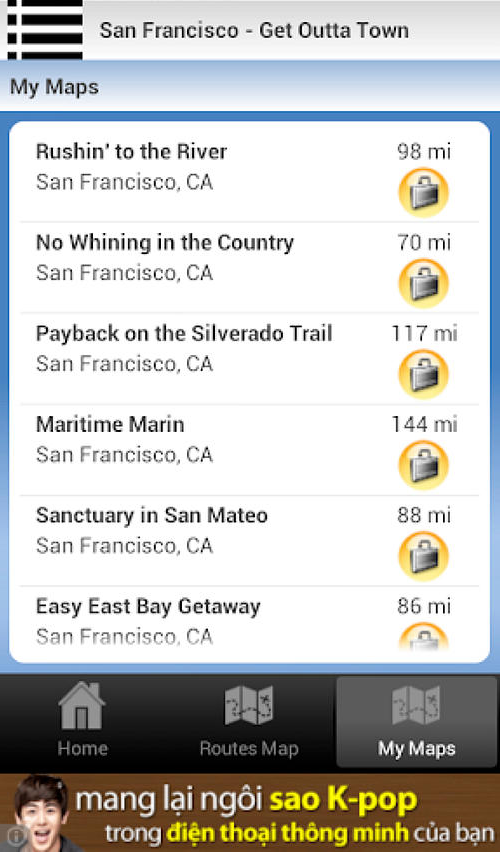
\includegraphics[width=0.65\textwidth]{images/mm-1.png}
			\caption{MADMAPS' Route Listing Page}
		\end{center}
	\end{minipage}
	\begin{minipage}{.49\textwidth}
		\begin{center}
			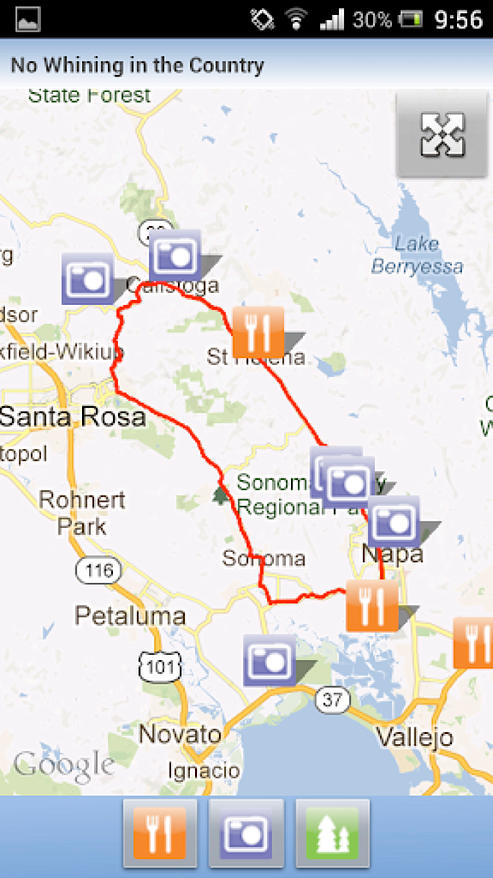
\includegraphics[width=0.625\textwidth]{images/mm-2.png}
			\caption{MADMAPS' Route Display Page}
		\end{center}
	\end{minipage}
\end{figure}

\subsection{MyScenicDrives} 
You can visit MyScenicDrives at \url{https://www.myscenicdrives.com/}
\begin{figure}[!ht]
	\centering
	\begin{minipage}{.49\textwidth}
		\begin{center}
			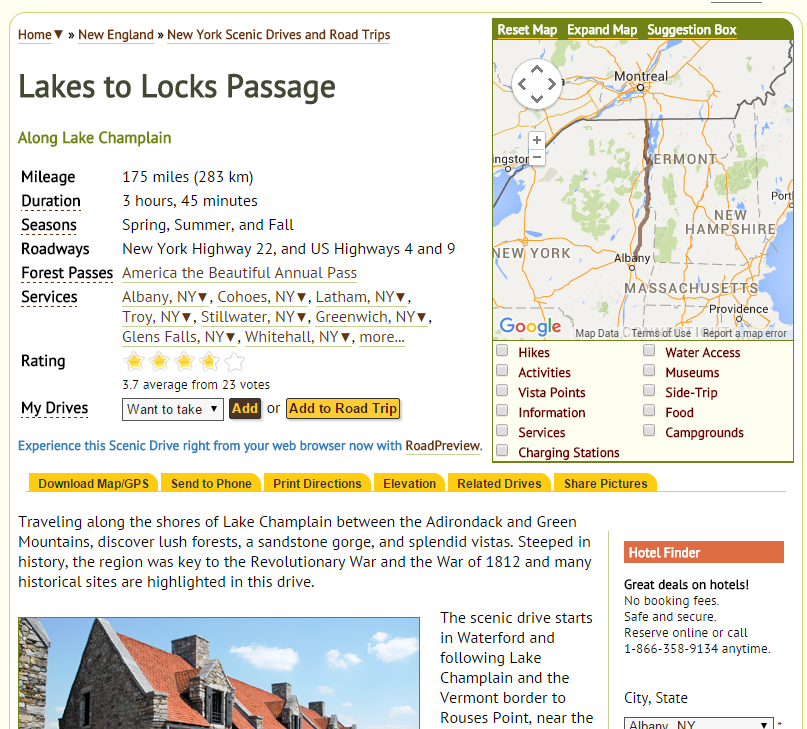
\includegraphics[width=0.95\textwidth]{images/msd-1.png}
			\caption{MyScenicDrive's Route detail page}
		\end{center}
	\end{minipage}
	\begin{minipage}{.49\textwidth}
		\begin{center}
			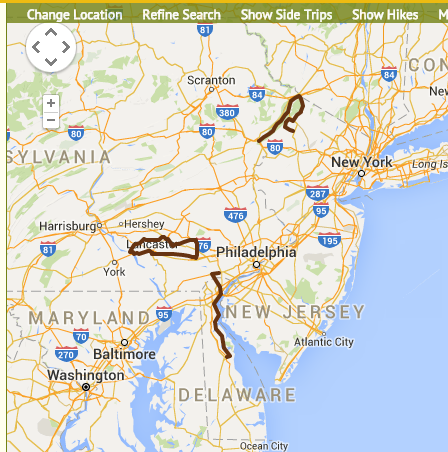
\includegraphics[width=0.9\textwidth]{images/msd-2.png}
			\caption{MyScenicDrive's Map Search Feature}
		\end{center}
	\end{minipage}
\end{figure}


\subsection{GoogleMaps ``My Maps''} 
You can visit Google's ``My Maps'' at \url{https://www.google.com/maps/d/}
\begin{figure}[!ht]
	\begin{center}
		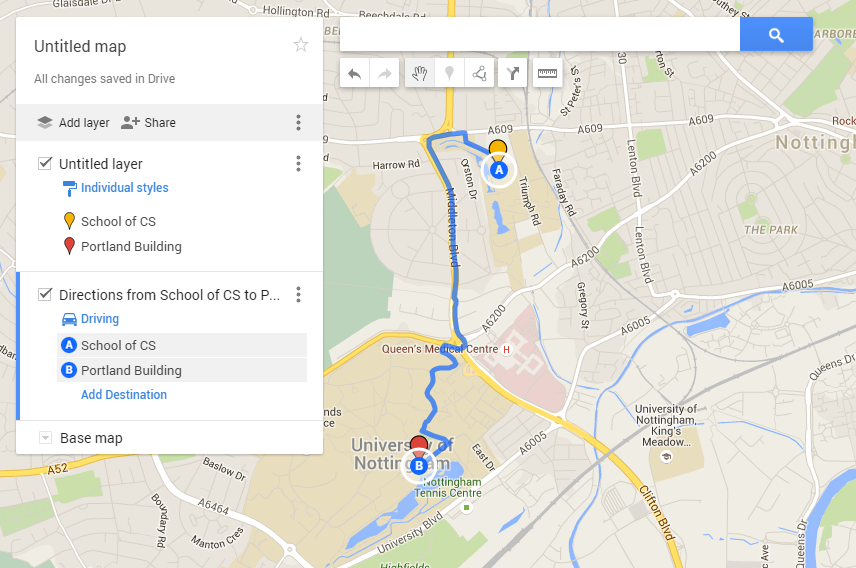
\includegraphics[width=0.7\textwidth]{images/google_maps.png}
	\end{center}
	\vspace{-6mm}
	\caption{Google Maps ``My Maps'' route creation page}
\end{figure}

\section{Initial Designs}
\label{app-designs}

\begin{figure}[!ht]
	\begin{center}
			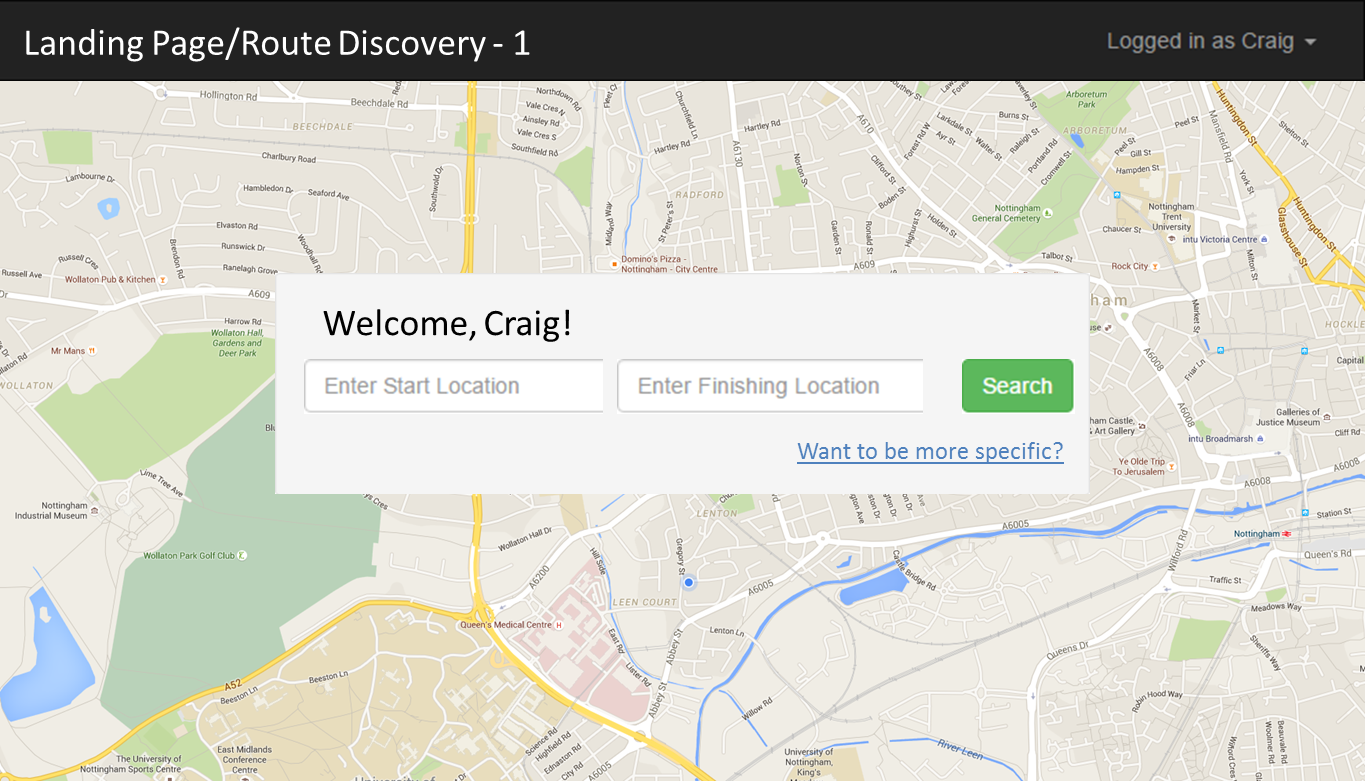
\includegraphics[width=0.99\textwidth]{images/ui-landing-1.png}
	\end{center}
	\vspace{-6mm}
	\caption{Initial landing page design}
\end{figure}
\newpage 
\begin{figure}[!ht]
	\begin{center}
			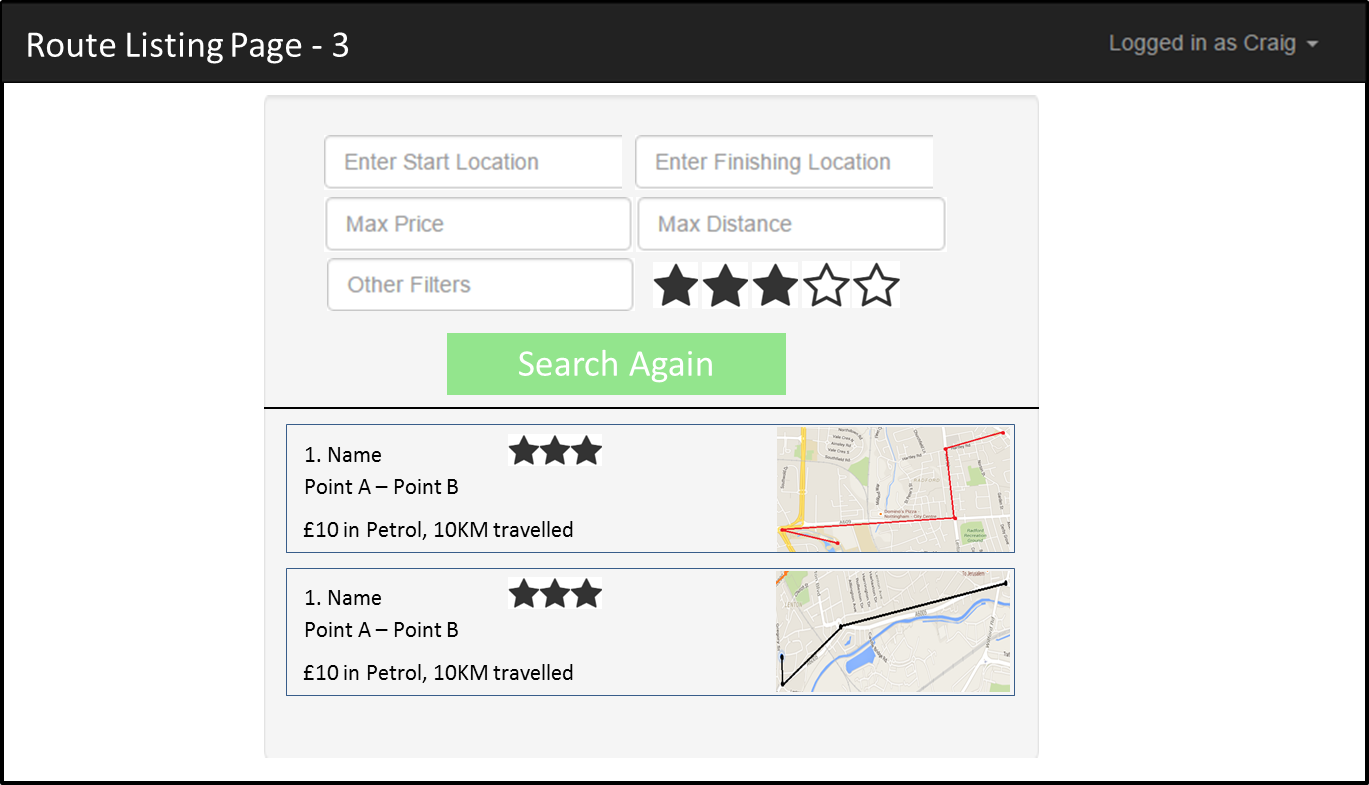
\includegraphics[width=0.99\textwidth]{images/ui-rlp-3.png}
	\end{center}
	\vspace{-6mm}
	\caption{Initial route listing page design}
\end{figure}
\begin{figure}[!ht]
	\begin{center}
			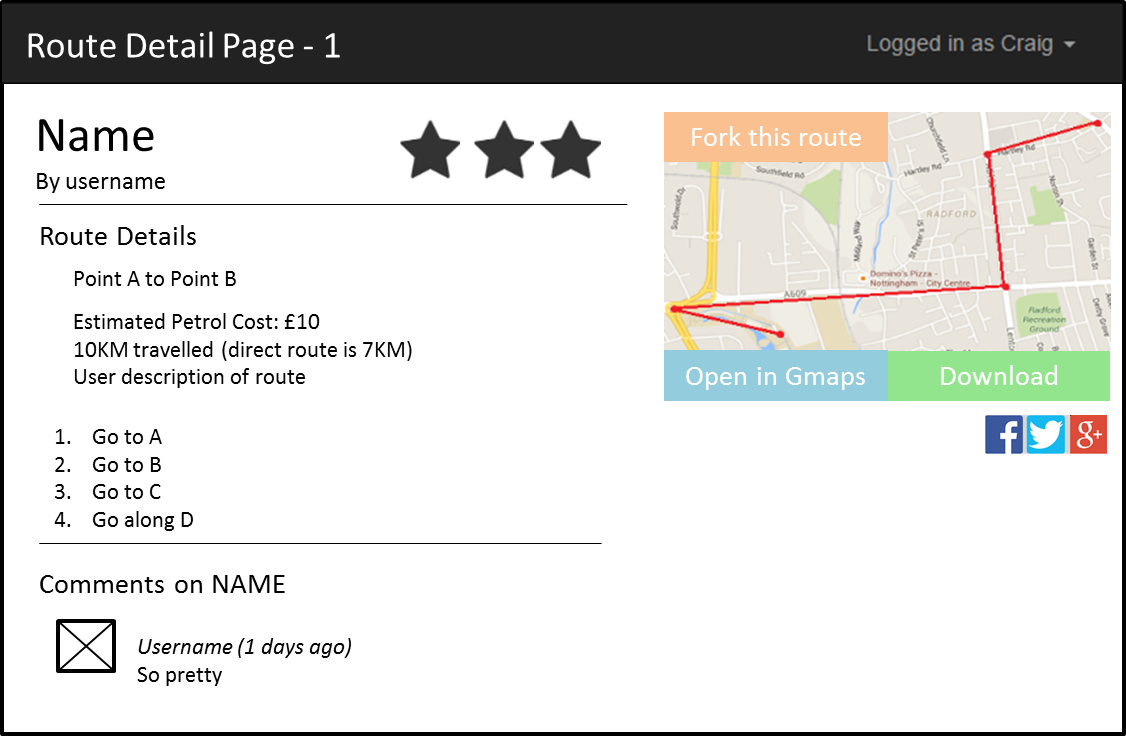
\includegraphics[width=0.99\textwidth]{images/ui-detail-1.png}
	\end{center}
	\vspace{-6mm}
	\caption{Initial route creation page design}
\end{figure}
\begin{figure}[!ht]
	\begin{center}
			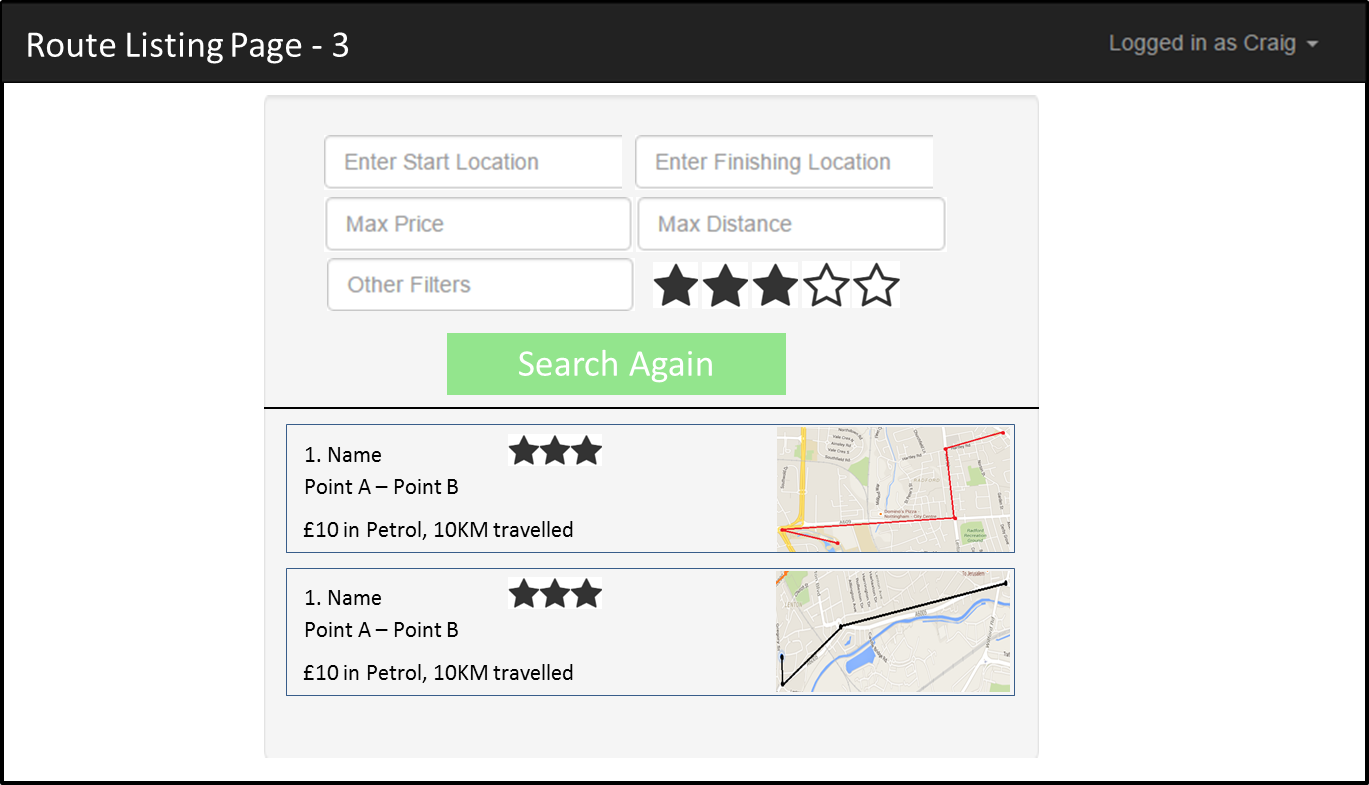
\includegraphics[width=0.99\textwidth]{images/ui-rlp-3.png}
	\end{center}
	\vspace{-6mm}
	\caption{Initial route detail page design}
\end{figure}

\newpage 
\section{System Flow Chart}
\label{app-sfc}
 \begin{figure}[!ht]
 	\begin{center}
 		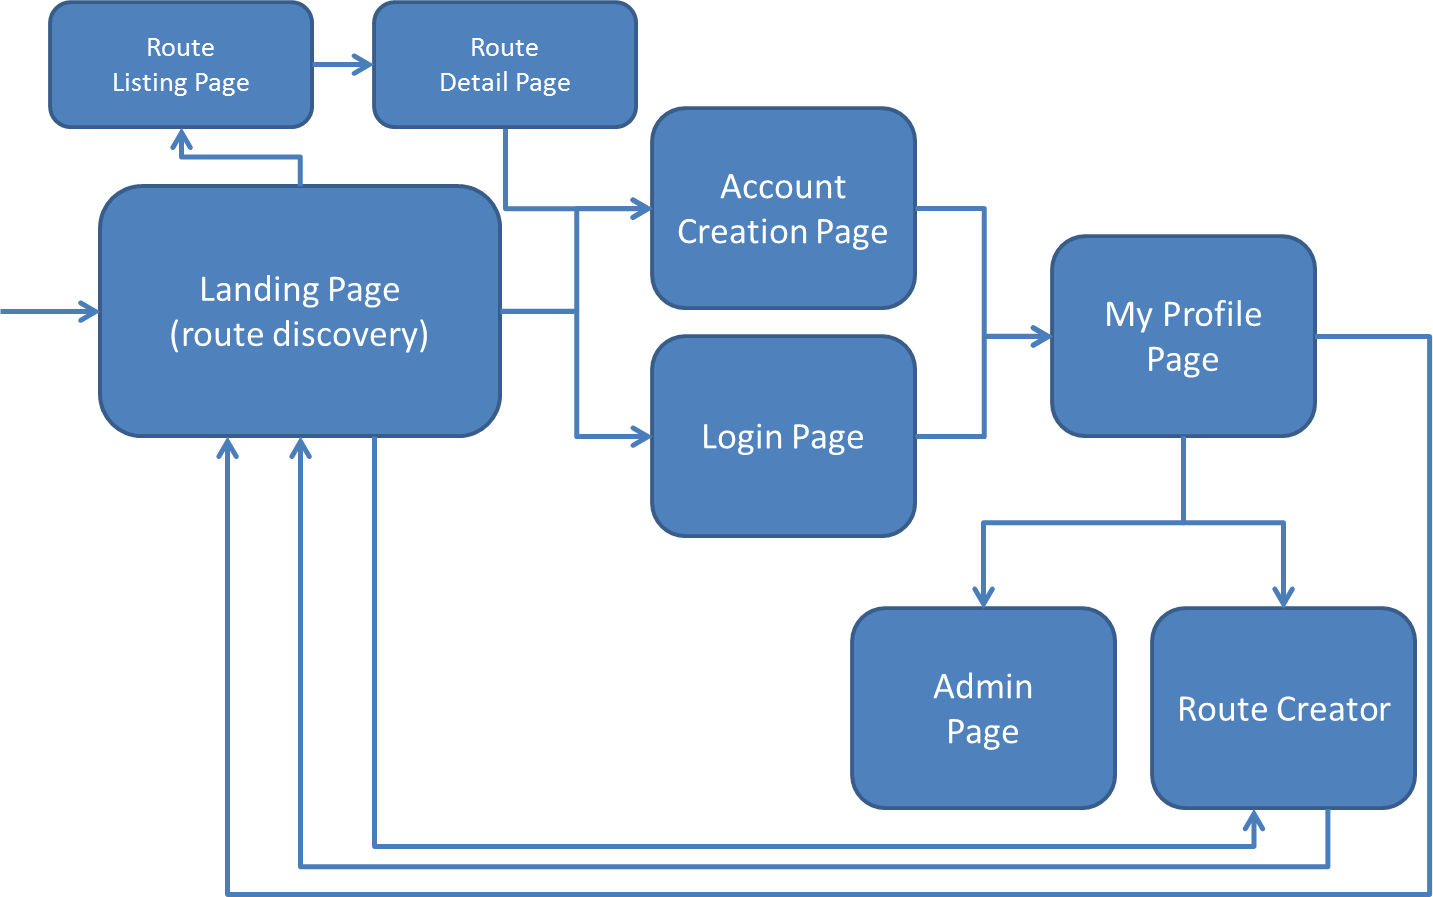
\includegraphics[width=0.9\textwidth]{images/flow.png}
 	\end{center}
 	\caption{System Flow Chart, detaiingl the user journey through the application}
 \end{figure}

\end{document}